\documentclass{standalone}
\usepackage{tikz}
\usetikzlibrary{patterns, positioning}


\begin{document}
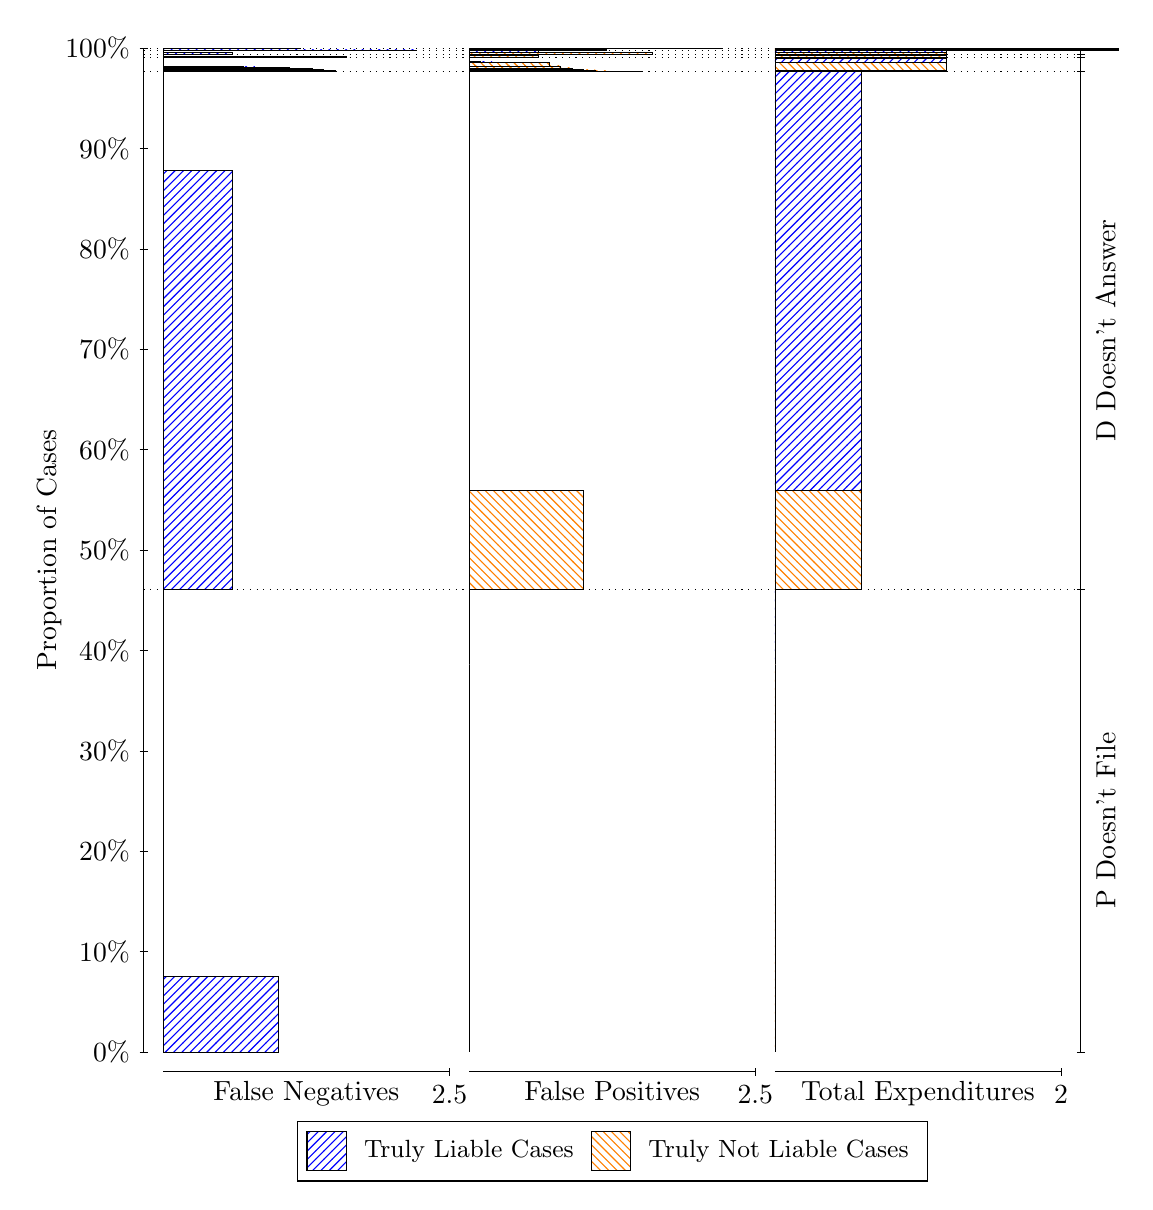
\begin{tikzpicture}
\draw[black, very thin] (1.5,1.75) -- (1.5,14.5);
\node[rotate=90, text=black, anchor=center] at (0.3, 8.125) {Proportion of Cases};
\draw[black, very thin] (1.45,1.75) -- (1.55,1.75);
\node[text=black, anchor=east] at (1.45, 1.75) {0\%};
\draw[black, very thin] (1.45,3.025) -- (1.55,3.025);
\node[text=black, anchor=east] at (1.45, 3.025) {10\%};
\draw[black, very thin] (1.45,4.3) -- (1.55,4.3);
\node[text=black, anchor=east] at (1.45, 4.3) {20\%};
\draw[black, very thin] (1.45,5.575) -- (1.55,5.575);
\node[text=black, anchor=east] at (1.45, 5.575) {30\%};
\draw[black, very thin] (1.45,6.85) -- (1.55,6.85);
\node[text=black, anchor=east] at (1.45, 6.85) {40\%};
\draw[black, very thin] (1.45,8.125) -- (1.55,8.125);
\node[text=black, anchor=east] at (1.45, 8.125) {50\%};
\draw[black, very thin] (1.45,9.4) -- (1.55,9.4);
\node[text=black, anchor=east] at (1.45, 9.4) {60\%};
\draw[black, very thin] (1.45,10.675) -- (1.55,10.675);
\node[text=black, anchor=east] at (1.45, 10.675) {70\%};
\draw[black, very thin] (1.45,11.95) -- (1.55,11.95);
\node[text=black, anchor=east] at (1.45, 11.95) {80\%};
\draw[black, very thin] (1.45,13.225) -- (1.55,13.225);
\node[text=black, anchor=east] at (1.45, 13.225) {90\%};
\draw[black, very thin] (1.45,14.5) -- (1.55,14.5);
\node[text=black, anchor=east] at (1.45, 14.5) {100\%};

\draw[black, very thin] (13.4,1.75) -- (13.4,14.5);
\draw[black, very thin] (13.35,1.75) -- (13.45,1.75);
\node[anchor=west] at (13.35, 1.75) {};
\draw[black, very thin] (13.35,7.6278) -- (13.45,7.6278);
\node[anchor=west] at (13.35, 7.6278) {};
\draw[black, very thin] (13.35,14.199) -- (13.45,14.199);
\node[anchor=west] at (13.35, 14.199) {};
\draw[black, very thin] (13.35,14.38) -- (13.45,14.38);
\node[anchor=west] at (13.35, 14.38) {};
\draw[black, very thin] (13.35,14.418) -- (13.45,14.418);
\node[anchor=west] at (13.35, 14.418) {};
\draw[black, very thin] (13.35,14.47) -- (13.45,14.47);
\node[anchor=west] at (13.35, 14.47) {};
\draw[black, very thin] (13.35,14.493) -- (13.45,14.493);
\node[anchor=west] at (13.35, 14.493) {};
\draw[black, very thin] (13.35,14.5) -- (13.45,14.5);
\node[anchor=west] at (13.35, 14.5) {};

\draw[black, very thin, pattern color=blue, pattern=north east lines] (1.75,1.75) rectangle (3.2033,2.7056);
\draw[black, very thin, pattern color=orange, pattern=north west lines] (1.75,2.7056) rectangle (1.75,7.6278);
\draw[black, very thin, pattern color=blue, pattern=north east lines] (1.75,7.6278) rectangle (2.622,12.942);
\draw[black, very thin, pattern color=orange, pattern=north west lines] (1.75,12.942) rectangle (1.75,14.199);
\draw[black, very thin, pattern color=blue, pattern=north east lines] (1.75,14.199) rectangle (3.93,14.217);
\draw[black, very thin, pattern color=blue, pattern=north east lines] (1.75,14.217) rectangle (3.7847,14.231);
\draw[black, very thin, pattern color=blue, pattern=north east lines] (1.75,14.231) rectangle (3.6393,14.24);
\draw[black, very thin, pattern color=blue, pattern=north east lines] (1.75,14.24) rectangle (3.494,14.246);
\draw[black, very thin, pattern color=blue, pattern=north east lines] (1.75,14.246) rectangle (3.3487,14.253);
\draw[black, very thin, pattern color=blue, pattern=north east lines] (1.75,14.253) rectangle (3.2033,14.256);
\draw[black, very thin, pattern color=blue, pattern=north east lines] (1.75,14.256) rectangle (3.058,14.259);
\draw[black, very thin, pattern color=blue, pattern=north east lines] (1.75,14.259) rectangle (2.9127,14.261);
\draw[black, very thin, pattern color=blue, pattern=north east lines] (1.75,14.261) rectangle (2.7673,14.263);
\draw[black, very thin, pattern color=orange, pattern=north west lines] (1.75,14.263) rectangle (1.75,14.38);
\draw[black, very thin, pattern color=blue, pattern=north east lines] (1.75,14.38) rectangle (4.0753,14.389);
\draw[black, very thin, pattern color=orange, pattern=north west lines] (1.75,14.389) rectangle (1.75,14.418);
\draw[black, very thin, pattern color=blue, pattern=north east lines] (1.75,14.418) rectangle (2.622,14.44);
\draw[black, very thin, pattern color=orange, pattern=north west lines] (1.75,14.44) rectangle (1.75,14.47);
\draw[black, very thin, pattern color=blue, pattern=north east lines] (1.75,14.47) rectangle (4.9473,14.475);
\draw[black, very thin, pattern color=orange, pattern=north west lines] (1.75,14.475) rectangle (1.75,14.493);
\draw[black, very thin, pattern color=blue, pattern=north east lines] (1.75,14.493) rectangle (3.494,14.497);
\draw[black, very thin, pattern color=orange, pattern=north west lines] (1.75,14.497) rectangle (1.75,14.5);
\draw[black, very thin, pattern color=orange, pattern=north west lines] (5.6333,1.75) rectangle (5.6333,6.6722);
\draw[black, very thin, pattern color=blue, pattern=north east lines] (5.6333,6.6722) rectangle (5.6333,7.6278);
\draw[black, very thin, pattern color=orange, pattern=north west lines] (5.6333,7.6278) rectangle (7.0867,8.884);
\draw[black, very thin, pattern color=blue, pattern=north east lines] (5.6333,8.884) rectangle (5.6333,14.199);
\draw[black, very thin, pattern color=orange, pattern=north west lines] (5.6333,14.199) rectangle (7.8133,14.2);
\draw[black, very thin, pattern color=orange, pattern=north west lines] (5.6333,14.2) rectangle (7.668,14.202);
\draw[black, very thin, pattern color=orange, pattern=north west lines] (5.6333,14.202) rectangle (7.5227,14.206);
\draw[black, very thin, pattern color=orange, pattern=north west lines] (5.6333,14.206) rectangle (7.3773,14.211);
\draw[black, very thin, pattern color=orange, pattern=north west lines] (5.6333,14.211) rectangle (7.232,14.222);
\draw[black, very thin, pattern color=orange, pattern=north west lines] (5.6333,14.222) rectangle (7.0867,14.231);
\draw[black, very thin, pattern color=orange, pattern=north west lines] (5.6333,14.231) rectangle (6.9413,14.248);
\draw[black, very thin, pattern color=orange, pattern=north west lines] (5.6333,14.248) rectangle (6.796,14.272);
\draw[black, very thin, pattern color=orange, pattern=north west lines] (5.6333,14.272) rectangle (6.6507,14.316);
\draw[black, very thin, pattern color=blue, pattern=north east lines] (5.6333,14.316) rectangle (6.36,14.317);
\draw[black, very thin, pattern color=blue, pattern=north east lines] (5.6333,14.317) rectangle (6.2147,14.319);
\draw[black, very thin, pattern color=blue, pattern=north east lines] (5.6333,14.319) rectangle (6.0693,14.322);
\draw[black, very thin, pattern color=blue, pattern=north east lines] (5.6333,14.322) rectangle (5.924,14.325);
\draw[black, very thin, pattern color=blue, pattern=north east lines] (5.6333,14.325) rectangle (5.7787,14.332);
\draw[black, very thin, pattern color=blue, pattern=north east lines] (5.6333,14.332) rectangle (5.6333,14.38);
\draw[black, very thin, pattern color=orange, pattern=north west lines] (5.6333,14.38) rectangle (6.5053,14.408);
\draw[black, very thin, pattern color=blue, pattern=north east lines] (5.6333,14.408) rectangle (5.6333,14.418);
\draw[black, very thin, pattern color=orange, pattern=north west lines] (5.6333,14.418) rectangle (7.9587,14.448);
\draw[black, very thin, pattern color=blue, pattern=north east lines] (5.6333,14.448) rectangle (6.5053,14.47);
\draw[black, very thin, pattern color=orange, pattern=north west lines] (5.6333,14.47) rectangle (7.3773,14.488);
\draw[black, very thin, pattern color=blue, pattern=north east lines] (5.6333,14.488) rectangle (5.924,14.493);
\draw[black, very thin, pattern color=orange, pattern=north west lines] (5.6333,14.493) rectangle (8.8307,14.496);
\draw[black, very thin, pattern color=blue, pattern=north east lines] (5.6333,14.496) rectangle (7.3773,14.5);
\draw[black, very thin, pattern color=orange, pattern=north west lines] (9.5167,1.75) rectangle (9.5167,6.6722);
\draw[black, very thin, pattern color=blue, pattern=north east lines] (9.5167,6.6722) rectangle (9.5167,7.6278);
\draw[black, very thin, pattern color=orange, pattern=north west lines] (9.5167,7.6278) rectangle (10.607,8.884);
\draw[black, very thin, pattern color=blue, pattern=north east lines] (9.5167,8.884) rectangle (10.607,14.199);
\draw[black, very thin, pattern color=orange, pattern=north west lines] (9.5167,14.199) rectangle (11.697,14.21);
\draw[black, very thin, pattern color=blue, pattern=north east lines] (9.5167,14.21) rectangle (11.697,14.217);
\draw[black, very thin, pattern color=orange, pattern=north west lines] (9.5167,14.217) rectangle (11.697,14.317);
\draw[black, very thin, pattern color=blue, pattern=north east lines] (9.5167,14.317) rectangle (11.697,14.368);
\draw[black, very thin, pattern color=orange, pattern=north west lines] (9.5167,14.368) rectangle (11.697,14.374);
\draw[black, very thin, pattern color=blue, pattern=north east lines] (9.5167,14.374) rectangle (11.697,14.38);
\draw[black, very thin, pattern color=orange, pattern=north west lines] (9.5167,14.38) rectangle (11.697,14.408);
\draw[black, very thin, pattern color=blue, pattern=north east lines] (9.5167,14.408) rectangle (11.697,14.418);
\draw[black, very thin, pattern color=orange, pattern=north west lines] (9.5167,14.418) rectangle (11.697,14.448);
\draw[black, very thin, pattern color=blue, pattern=north east lines] (9.5167,14.448) rectangle (11.697,14.47);
\draw[black, very thin, pattern color=orange, pattern=north west lines] (9.5167,14.47) rectangle (13.877,14.488);
\draw[black, very thin, pattern color=blue, pattern=north east lines] (9.5167,14.488) rectangle (13.877,14.493);
\draw[black, very thin, pattern color=orange, pattern=north west lines] (9.5167,14.493) rectangle (13.877,14.496);
\draw[black, very thin, pattern color=blue, pattern=north east lines] (9.5167,14.496) rectangle (13.877,14.5);
\draw[black, dotted] (1.5,7.6278) -- (13.4,7.6278);
\draw[black, dotted] (1.5,14.199) -- (13.4,14.199);
\draw[black, dotted] (1.5,14.38) -- (13.4,14.38);
\draw[black, dotted] (1.5,14.418) -- (13.4,14.418);
\draw[black, dotted] (1.5,14.47) -- (13.4,14.47);
\draw[black, dotted] (1.5,14.493) -- (13.4,14.493);
\draw[black, very thin] (1.75,1.5) -- (5.3833,1.5);
\node[text=black, anchor=north] at (3.5667, 1.5) {False Negatives};
\draw[black, very thin] (5.3833,1.45) -- (5.3833,1.55);
\node[text=black, anchor=north] at (5.3833, 1.45) {2.5};

\draw[black, very thin] (5.6333,1.5) -- (9.2667,1.5);
\node[text=black, anchor=north] at (7.45, 1.5) {False Positives};
\draw[black, very thin] (9.2667,1.45) -- (9.2667,1.55);
\node[text=black, anchor=north] at (9.2667, 1.45) {2.5};

\draw[black, very thin] (9.5167,1.5) -- (13.15,1.5);
\node[text=black, anchor=north] at (11.333, 1.5) {Total Expenditures};
\draw[black, very thin] (13.15,1.45) -- (13.15,1.55);
\node[text=black, anchor=north] at (13.15, 1.45) {2};

\node[text=black, centered, rotate=90] at (13.72, 4.6889) {P Doesn't File};
\node[text=black, centered, rotate=90] at (13.72, 10.913) {D Doesn't Answer};






\draw (7.449999999999999,1.5) node[draw=none] (baseCoordinate) {};
\begin{scope}[align=center]
        \matrix[scale=0.5, draw=black, below=0.5cm of baseCoordinate, nodes={draw}, column sep=0.1cm]{
            \node[rectangle, draw, minimum width=0.5cm, minimum height=0.5cm, pattern color=blue, pattern=north east lines] {}; &
            \node[draw=none, font=\small, text=black] (B) {Truly Liable Cases}; &
            \node[rectangle, draw, minimum width=0.5cm, minimum height=0.5cm, pattern color=orange, pattern=north west lines] {}; &
            \node[draw=none, font=\small, text=black] (B) {Truly Not Liable Cases}; \\
            };
\end{scope}

\end{tikzpicture}
\end{document}